\documentclass{article}
\usepackage{graphicx}
\usepackage{listings}
\usepackage{xcolor}
\usepackage{hyperref}
\usepackage[a4paper, top=2cm, bottom=1.5cm, left=2.5cm, right=2.5cm]{geometry}
\begin{document}
\lstdefinelanguage{RISC-V}{
  morekeywords=[1]{
    add, addi, and, andi, auipc, beq, bge, bgeu, blt, bltu, bne, jal, jalr, lb, lbu, lh, lhu, lui, lw, or, ori, sb, sh, sll, slli, slt, slti, sltiu, sltu, sra, srai, srl, srli, sub, sw, xor, xori
  },
  morekeywords=[2]{
    .align, .ascii, .asciiz, .byte, .data, .double, .extern, .float, .global, .half, .space, .text, .word
  },
  sensitive=true,
  morecomment=[l]{\#},
  morestring=[b]",
  morestring=[b]',
}
\definecolor{lightgreen}{RGB}{230, 255, 230}
\lstdefinestyle{mystyle}{
    backgroundcolor=\color{lightgreen},
    basicstyle=\ttfamily\small,
    keywordstyle=\bfseries\color{blue},
    commentstyle=\itshape\color{gray},
    stringstyle=\color{orange},
    numbers=left,
    numbersep=5pt,
    numberstyle=\tiny\color{gray},
    breaklines=true,
    showstringspaces=false,
    tabsize=4
}
\lstset{style=mystyle}
\begin{center}
    {
\includegraphics[width=10cm]{LOGOHABIB.png} \\
    \vspace{10mm}}
    {\Large CE/CS 321/330 Computer Architecture} \\
    \vspace{10mm}
    {\Large Spring 2024} \\
    \vspace{10mm}
    {\huge \textbf{Final Lab Project}} \\
    \vspace{7mm}
    {\Large \textbf{5-Stage Pipelined Processor To Execute A Single Array Sorting Algorithm}} \\
    \vspace{20mm}
    {\Large \textbf{Group Members}} \\
    \vspace{5mm}
    {\Large Bilal Ahmed (ba08018)} \\
    \vspace{5mm}
    {\Large Hammad Malik (hm08298)} \\
    \vspace{5mm}
    {\Large Ahtisham Uddin (au08429)} \\
    \vspace{5mm}
\end{center}
\pagebreak
\tableofcontents
\pagebreak

\section{Introduction}
\hspace{1cm} The purpose of this project is to design a 5-stage pipelined processor to execute a single array sorting algorithm. We will be converting our single cycle
processor to a pipelined one. The processor is designed in Verilog HDL and
the sorting algorithm is written in RISC-V assembly language. The processor
is first executed using single cycle processor, it is then implemented by adding
in pipelining to the processor to increase efficiency in our processor. The report
is divided according to each task that we had to implement according to the
project rubrics.

\section{Methodology}
\subsection{Task 1}
\subsubsection{Risc V Assemby Code for Bubble Sort}
\hspace{1cm} We implemented \textbf{"Bubble Sort"} sorting algorithm in RISC V assembly on the Venus simulator.  
\begin{lstlisting}[caption={Selection Sort Assembly code}, captionpos=b, language=RISC-V]
addi x18, x0, 0 #to track a[i] offset

add x8, x0, x0 # i iterator (starts at 0)
outerloop: beq x8, x11, outerexit #i < 10
add x29, x0, x8 # j iterator (set to i each outer loop)

add x19, x8, x0
add x19, x19, x19
add x19, x19, x19

innerloop: beq x29, x11, innerexit #j < 10

addi x29, x29, 1 # increment j by 1
addi x19, x19, 8 # increment j offset

lw x26, 0x0(x18)     # load a[i] into register
lw x27, 0x0(x19)     # load a[j] into register

blt x26, x27, bubblesort # if a[i] < a[j], dont restart loop but bubble sort

beq x0,x0, innerloop # unconditional loop

bubblesort: 
add x5, x0, x26 # int temp = a[i]
sw x27, 0(x18) # a[i] = a[j]
sw x5, 0(x19) # a[j] = temp

beq x0, x0, innerloop # restart j
innerexit:

addi x8, x8, 1 #increment i
addi, x18, x18, 8 # increment i offset
beq x0, x0, outerloop
outerexit:
    

\end{lstlisting}
\subsubsection{Bubble Sort Implementation}
\hspace{1cm} We made modifications to the lab 11 module where all modules were instantiated together to make a processor. We revised the ALU and instruction memory code, incorporating a branch unit code to facilitate branch operations. In the ALU code, we introduced functionality for the funct3 bit of bgt and blt, and expanded the 4-byte offset to an 8-byte offset to accommodate our 64-bit processor. Additionally, we initialized a list and sorted it using the instruction memory on the single-cycle processor. We made changes to Data Memory too, adding on the data to be sorted.
\pagebreak
\subsubsection{Result}
\begin{figure} [ht]
    \centering 
    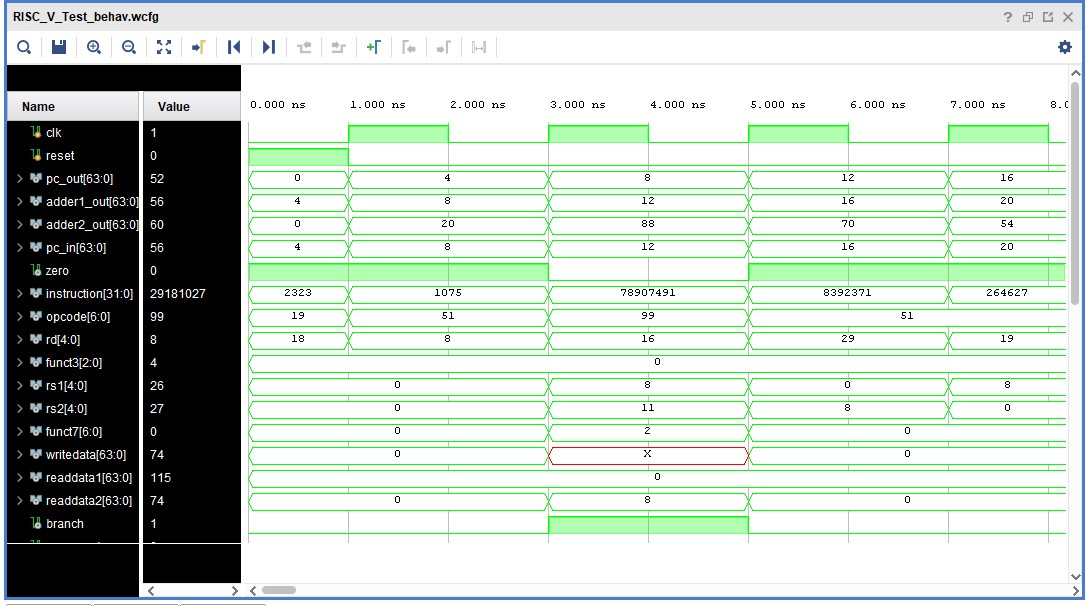
\includegraphics[width=1\textwidth]{task 1 simulation.jpg} 
    \caption{Simulation Output} 
    \label{fig:Output 1} 
\end{figure}
\begin{figure} 
    \centering 
    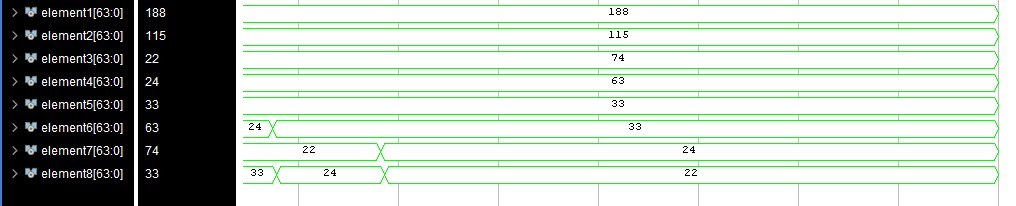
\includegraphics[width=1\textwidth]{task 1 sorted array.jpg} 
    \caption{Sorted Array} 
    \label{fig:Array 1} 
\end{figure}
\pagebreak
\subsection{Changes in Code}
\subsubsection{Instruction Memory}
\begin{lstlisting}[caption={Design Module for Instruction Memory}, captionpos=b, language=RISC-V]
module Instruction_Memory
(
input [63:0] Inst_Address,
output reg [31:0] Instruction
);
reg [7:0] inst_mem [87:0];
initial
begin
      {inst_mem[3], inst_mem[2], inst_mem[1], inst_mem[0]} = 32'h00000913;//1
      {inst_mem[7], inst_mem[6], inst_mem[5], inst_mem[4]} = 32'h00000433;//2
      {inst_mem[11], inst_mem[10], inst_mem[9], inst_mem[8]} = 32'h04b40863;//3
      {inst_mem[15], inst_mem[14], inst_mem[13], inst_mem[12]} = 32'h00800eb3;//4
      {inst_mem[19], inst_mem[18], inst_mem[17], inst_mem[16]} = 32'h000409b3;//5	
      {inst_mem[23], inst_mem[22], inst_mem[21], inst_mem[20]} = 32'h013989b3;//6
      {inst_mem[27], inst_mem[26], inst_mem[25], inst_mem[24]} = 32'h013989b3;//7
      {inst_mem[31], inst_mem[30], inst_mem[29], inst_mem[28]} = 32'h013989b3;//8
      {inst_mem[35], inst_mem[34], inst_mem[33], inst_mem[32]} = 32'h02be8663;//9
      {inst_mem[39], inst_mem[38], inst_mem[37], inst_mem[36]} = 32'h001e8e93;//10	
      {inst_mem[43], inst_mem[42], inst_mem[41], inst_mem[40]} = 32'h00898993;//11
      {inst_mem[47], inst_mem[46], inst_mem[45], inst_mem[44]} = 32'h00093d03;//12
      {inst_mem[51], inst_mem[50], inst_mem[49], inst_mem[48]} = 32'h0009bd83;//13
      {inst_mem[55], inst_mem[54], inst_mem[53], inst_mem[52]} = 32'h01bd4463;//14
      {inst_mem[59], inst_mem[58], inst_mem[57], inst_mem[56]} = 32'hfe0004e3;//15
      {inst_mem[63], inst_mem[62], inst_mem[61], inst_mem[60]} = 32'h01a002b3;//16
      {inst_mem[67], inst_mem[66], inst_mem[65], inst_mem[64]} = 32'h01b93023;//17
      {inst_mem[71], inst_mem[70], inst_mem[69], inst_mem[68]} = 32'h0059b023;//18
      {inst_mem[75], inst_mem[74], inst_mem[73], inst_mem[72]} = 32'hfc000ce3;//19
      {inst_mem[79], inst_mem[78], inst_mem[77], inst_mem[76]} = 32'h00140413;//20
      {inst_mem[83], inst_mem[82], inst_mem[81], inst_mem[80]} = 32'h00890913;//21
      {inst_mem[87], inst_mem[86], inst_mem[85], inst_mem[84]} = 32'hfa000ae3;//22
end
always @(Inst_Address)
begin
Instruction[7:0] = inst_mem[Inst_Address+0];
      Instruction[15:8] = inst_mem[Inst_Address+1];
      Instruction[23:16] = inst_mem[Inst_Address+2];
      Instruction[31:24] = inst_mem[Inst_Address+3];
end
endmodule
\end{lstlisting}
\subsubsection{Data Memory Memory}
\begin{lstlisting}[caption={Design Module for Data Memory}, captionpos=b, language=RISC-V]
module Data_Memory
(
input [63:0] Mem_Addr,
input [63:0] Write_Data,
input clk, MemWrite, MemRead,
output reg [63:0] Read_Data,
output [63:0] element1,
  output [63:0] element2,
  output [63:0] element3,
  output [63:0] element4,
  output [63:0] element5,
  output [63:0] element6,
  output [63:0] element7,
  output [63:0] element8
);
reg [7:0] DataMemory [255:0];
integer i;
initial
begin
for (i = 0;i<256;i = i + 1)begin
    DataMemory[i] = 0;
end
      DataMemory[0] = 8'd188;
      DataMemory[8] = 8'd22;
      DataMemory[16] = 8'd33;
      DataMemory[24] = 8'd24;
      DataMemory[32] = 8'd115;
      DataMemory[40] = 8'd63;
      DataMemory[48] = 8'd74;
      DataMemory[56] = 8'd33;
end

  assign element1 = {DataMemory[7],DataMemory[6],DataMemory[5],DataMemory[4],DataMemory[3],DataMemory[2],DataMemory[1],DataMemory[0]};
  assign element2 = {DataMemory[15],DataMemory[14],DataMemory[13],DataMemory[12],DataMemory[11],DataMemory[10],DataMemory[9],DataMemory[8]};
  assign element3 = {DataMemory[23],DataMemory[22],DataMemory[21],DataMemory[20],DataMemory[19],DataMemory[18],DataMemory[17],DataMemory[16]};
  assign element4 = {DataMemory[31],DataMemory[30],DataMemory[29],DataMemory[28],DataMemory[27],DataMemory[26],DataMemory[25],DataMemory[24]};
  assign element5 = {DataMemory[39],DataMemory[38],DataMemory[37],DataMemory[36],DataMemory[35],DataMemory[34],DataMemory[33],DataMemory[32]};
  assign element6 = {DataMemory[47],DataMemory[46],DataMemory[45],DataMemory[44],DataMemory[43],DataMemory[42],DataMemory[41],DataMemory[40]};
  assign element7 = {DataMemory[55],DataMemory[54],DataMemory[53],DataMemory[52],DataMemory[51],DataMemory[50],DataMemory[49],DataMemory[48]};
  assign element8 = {DataMemory[63],DataMemory[62],DataMemory[61],DataMemory[60],DataMemory[59],DataMemory[58],DataMemory[57],DataMemory[56]};


always @ (*)
begin
if (MemRead)
Read_Data =
{DataMemory[Mem_Addr+7],DataMemory[Mem_Addr+6],DataMemory[Mem_Addr+5],DataMemory[Mem_Addr+4],DataMemory[Mem_Addr+3],DataMemory[Mem_Addr+2],DataMemory[Mem_Addr+1],DataMemory[Mem_Addr]};
end
always @ (posedge clk)
begin
if (MemWrite)
begin
DataMemory[Mem_Addr] = Write_Data[7:0];
DataMemory[Mem_Addr+1] = Write_Data[15:8];
DataMemory[Mem_Addr+2] = Write_Data[23:16];
DataMemory[Mem_Addr+3] = Write_Data[31:24];
DataMemory[Mem_Addr+4] = Write_Data[39:32];
DataMemory[Mem_Addr+5] = Write_Data[47:40];
DataMemory[Mem_Addr+6] = Write_Data[55:48];
DataMemory[Mem_Addr+7] = Write_Data[63:56];
end
end
endmodule
\end{lstlisting}
\subsubsection{Branching Unit}
\begin{lstlisting}[caption={Design Module for Branching Unit}, captionpos=b, language=RISC-V]
module branching_unit
  (
   input [2:0] funct3,
    input [63:0] readData1,
    input [63:0] b,
   output reg addermuxselect
  );
  
  initial
    begin
      addermuxselect = 1'b0;
    end
  
  always @(*)
	begin
      case (funct3)
        3'b000:
          begin
            if (readData1 == b)
              addermuxselect = 1'b1;
            else
              addermuxselect = 1'b0;
            end
         3'b100:
    		begin
              if (readData1 < b)
              addermuxselect = 1'b1;
            else
              addermuxselect = 1'b0;
            end
        3'b101:
          begin
            if (readData1 > b)
          	addermuxselect = 1'b1;
           else
              addermuxselect = 1'b0;
          end    
      endcase
     end
endmodule
\end{lstlisting}
\subsection{Task 2}
\subsubsection{Pipelined Processor}
\hspace{1cm} A difficulty with implementation of single cycle processor is that the processor only executes one instruction at a time, and only after that instruction is finished is execution of the subsequent instruction begins, which is counter-productive. Given that the majority of the components in our processors would remain idle, it is immediately clear how wasteful this would be and how much processing power it would waste. This is why, in this section, we'll try to fix it by adding pipelining to our single-cycle processor.

\hspace{1cm}Pipelining would allow us to execute numerous commands at once. An in-depth explanation of how this works will be provided in the following section, but for now, consider that one component will work on one portion of the instruction while the other will work on a different part at the same point, thus increasing the efficiency of the whole program. We`ll be incorporating a five-stage pipeline into our Risc-V processor, allowing it to handle five instructions at once. The five stages we implemented for the processor are as follows:

\begin{enumerate}
    \item IF: Instruction Fetch
    \item ID: Instruction Decode 
    \item EX: Execution or address calculation
    \item MEM: Data Memory Access
    \item WB: Write back

\end{enumerate}

We will be introducing four new registers to implement the pipelining stage and to make our program more efficient. These registers are as follows:

\begin{enumerate}
    \item IF/ID register: This register will be used to store the instruction fetched in the IF stage and will be used in the ID stage.
    \item ID/EX register: This register will be used to store the instruction decoded in the ID stage and will be used in the EX stage.
    \item EX/MEM register: This register stores the result of the execution stage.
    \item MEM/WB register: This register stores the result of the memory access stage.
\end{enumerate}

These four newly introduced pipeline registers help in the pipelining process. These registers allow the pipeline to handle multiple instructions simultaneously and keep track of the progress of each instruction as it moves through the pipeline. The use of these registers helps to improve the performance of the processor by enabling the processing of multiple instructions in parallel.

An ideal pipeline would be one which continously moves forward and the instructions are only provided and moved forward. However, this is not the case with the pipeline taught to us. e of the PC, choosing between the
incremented PC and the branch address from the MEM stage. 

Along with the four intermediate pipeline registers, we will also add a control line and a forwarding unit. We extend these registered to store the control lines passed from one stage to another. These registers would be timed to the clock and would either send the stored contents for additional processing or be flushed on each positive edge.

\subsubsection{Result}

\begin{figure} [h]
    \centering 
    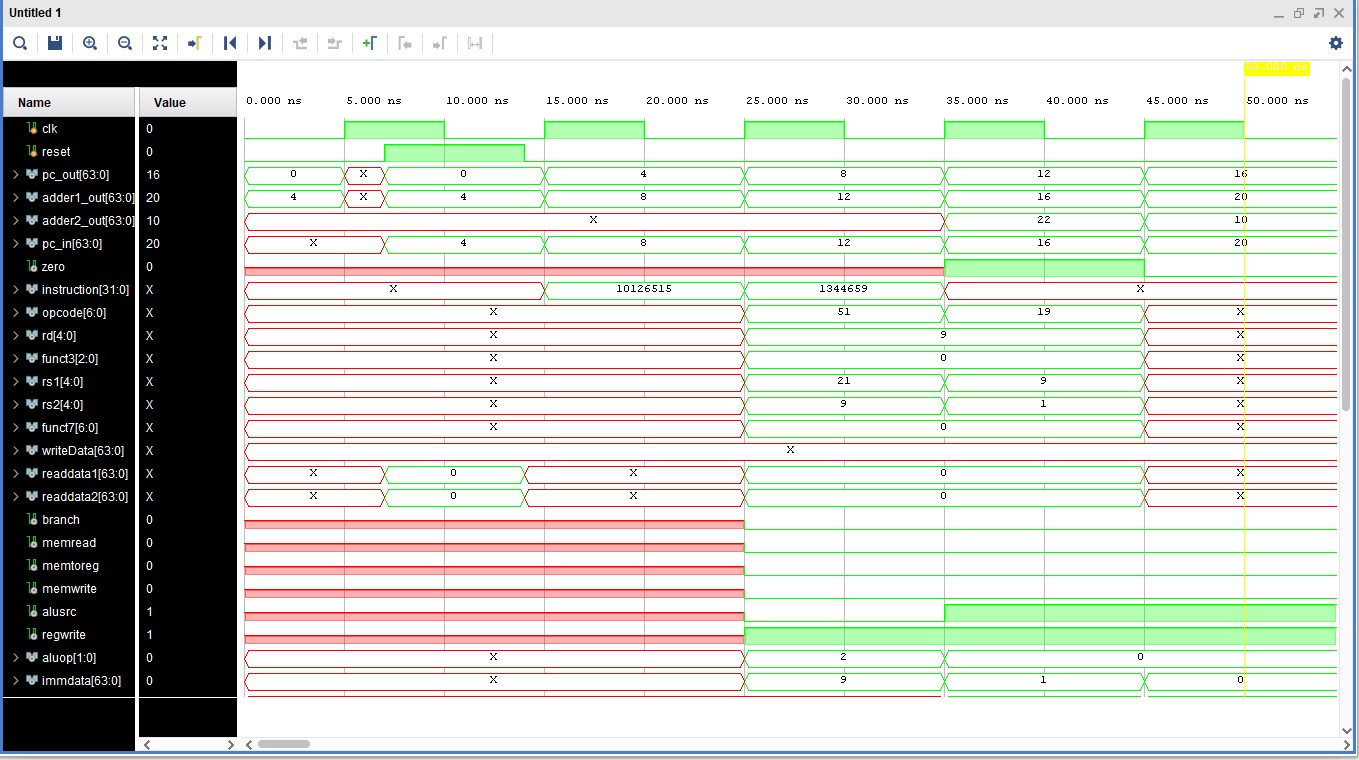
\includegraphics[width=1\textwidth]{task 2 simulation.jpg} 
    \caption{Simulation Output} 
    \label{fig:Output 2} 
\end{figure}
\begin{figure} [h]
    \centering 
    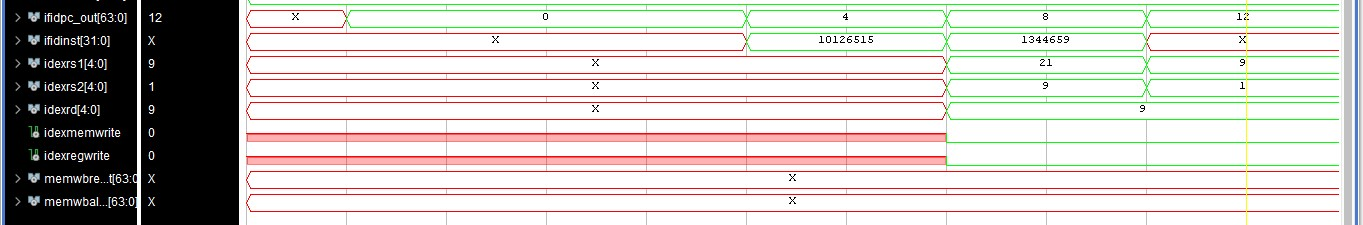
\includegraphics[width=1\textwidth]{task 2 forwarding.jpg} 
    \caption{Forwarding Output} 
    \label{fig:Output 3} 
\end{figure}
\subsection{Code Changes}
\subsubsection{IF/ID}
\begin{lstlisting}[caption={Design Module for IF/ID}, captionpos=b, language=RISC-V]
module ifidreg(
input clk,
input reset,
input [63:0] pc_out,
input [31:0] instruction,
output reg [63:0] ifidpc_out,
output reg [31:0] ifidinst);

always @(posedge clk) begin
    if (reset == 1'b1) begin
        ifidpc_out = 0;
        ifidinst = 0;
        end
    else begin
        ifidpc_out = pc_out;
        ifidinst = instruction;
        end
end

endmodule
\end{lstlisting}
\subsubsection{ID/EX}
\begin{lstlisting}[caption={Design Module for ID/EX}, captionpos=b, language=RISC-V]
module idexreg(
input clk,
input reset,
input  [63:0] ifidpc_out, readdata1, readdata2, imm,
input  [4:0] rs1, rs2, rd,
input  [3:0] funct3,
input  branch, memread, memtoreg, memwrite, regwrite, alusrc,
input  [1:0] aluop,
output reg [63:0]idexpc_out, idexreaddata1, idexreaddata2, ideximm,
output reg [4:0] idexrs1, idexrs2, idexrd,
output reg [3:0] idexfunct3,
output reg idexbranch, idexmemread, idexmemtoreg, idexmemwrite, idexregwrite, idexalusrc,
output reg [1:0] idexaluop
    );
    
always @(posedge clk) begin
    if (reset == 1'b1)begin
        idexpc_out = 0;
        idexreaddata1 = 0;
        idexreaddata2 = 0;
        ideximm = 0;
        idexrs1 = 0;
        idexrs2 = 0;
        idexrd = 0;
        idexfunct3 = 0;
        idexbranch = 0;
        idexmemread = 0;
        idexmemtoreg = 0;
        idexmemwrite = 0;
        idexregwrite = 0;
        idexalusrc = 0;
        idexaluop = 0;
        end
    else begin
        idexpc_out = ifidpc_out;
        idexreaddata1 = readdata1;
        idexreaddata2 = readdata2;
        ideximm = imm;
        idexrs1 = rs1;
        idexrs2 = rs2;
        idexrd = rd;
        idexfunct3 = funct3;
        idexbranch = branch;
        idexmemread = memread;
        idexmemtoreg = memtoreg;
        idexmemwrite = memwrite;
        idexregwrite = memwrite;
        idexalusrc = alusrc;
        idexaluop = aluop;
        end
        
    end
endmodule
\end{lstlisting}

\subsubsection{EX/MEM}
\begin{lstlisting}[caption={Design Module for EX/MEM}, captionpos=b, language=RISC-V]
module exmemreg(
  input clk,reset,
  input [63:0] adderout, //adder output
  input [63:0] resultinalu,//64bit alu output
  input zeroin,//64bit alu output
  input [63:0] writedatain, //2 bit mux2by1 output
  input [4:0] rdin, //IDEX output
  input branchin,memreadin, memtoregin, memwritein, regwritein, //IDEXX outputs
  input addermuxselectin,
  output reg [63:0] exmemadderout,
  output reg exmemzero,
  output reg [63:0] exmemresultoutalu,
  output reg [63:0] exmemwritedataout,
  output reg [4:0] exmemrd,
  output reg exmembranch, exmemmemread, exmemmemtoreg, exmemmemwrite, exmemregwrite,
  output reg exmemaddermuxselect);
  
  always @(posedge clk)
    begin
      if (reset == 1'b1)
        begin
          exmemadderout = 64'b0;
          exmemzero = 1'b0;
          exmemresultoutalu = 63'b0;
          exmemwritedataout = 64'b0;
          exmemrd = 5'b0;
          exmembranch = 1'b0;
          exmemmemread = 1'b0;
          exmemmemtoreg =1'b0;
          exmemmemwrite = 1'b0;
          exmemregwrite = 1'b0;
          exmemaddermuxselect = 1'b0;
        end
      else
        begin
          exmemadderout = adderout;
          exmemzero = zeroin;
          exmemresultoutalu = resultinalu;
          exmemwritedataout = writedatain;
          exmemrd = rdin;
          exmembranch = branchin;
          exmemmemread = memreadin;
          exmemmemtoreg = memtoregin;
          exmemmemwrite = memwritein;
          exmemregwrite = regwritein;
          exmemaddermuxselect = addermuxselectin;
        end
    end
endmodule
\end{lstlisting}

\subsubsection{MEM/WB}
\begin{lstlisting}[caption={Design Module for MEM/WB}, captionpos=b, language=RISC-V]
module memwbreg(
input clk,reset,
  input [63:0] read_data_in,
  input [63:0] result_alu_in, //2 bit 2by1 mux input b
  input [4:0] Rd_in, //EX MEM output
  input memtoreg_in, regwrite_in, //ex mem output as mem wb inputs
  output reg [63:0] readdata, //1bit
  output reg [63:0] result_alu_out,//1bit
  output reg [4:0] rd,
  output reg Memtoreg, Regwrite
);
  
  always @(posedge clk)
    begin
      if (reset == 1'b1)
        begin
          readdata = 63'b0;
          result_alu_out = 63'b0;
          rd = 5'b0;
          Memtoreg = 1'b0;
          Regwrite = 1'b0;
          
        end
      else
        begin
         readdata = read_data_in;
          result_alu_out = result_alu_in;
          rd = Rd_in;
          Memtoreg = memtoreg_in;
          Regwrite = regwrite_in;
        end
    end
endmodule
\end{lstlisting}

\subsubsection{Forwarding Unit}
\begin{lstlisting}[caption={Design Module for Forwarding Unit}, captionpos=b, language=RISC-V]
   module forwardingunit
  (
    input [4:0] RS_1, //ID/EX.RegisterRs1
    input [4:0] RS_2, //ID/EX.RegisterRs2
    input [4:0] rdMem, //EX/MEM.Register Rd
    input [4:0] rdWb, //MEM/WB.RegisterRd
    
    input regWrite_Wb, //MEM/WB.RegWrite
    input regWrite_Mem, // EX/MEM.RegWrite
    output reg [1:0] Forward_A,
    output reg [1:0] Forward_B
 );
  
  always @(*)
    begin
    	if ( (rdMem == RS_1) & (regWrite_Mem != 0 & rdMem !=0))
          begin
          	Forward_A = 2'b10;
          end
      	else
          begin 
            // Not condition for MEM hazard 
            if ((rdWb== RS_1) & (regWrite_Wb != 0 & rdWb != 0) & ~((rdMem == RS_1) &(regWrite_Mem != 0 & rdMem !=0)  )  )
              begin
                Forward_A = 2'b01;
              end
            else
              begin
                Forward_A = 2'b00;
              end
          end
      
        if ( (rdMem == RS_2) & (regWrite_Mem != 0 & rdMem !=0) )
          begin
            Forward_B = 2'b10;
          end
        else
          begin
            // Not condition for MEM Hazard 
            if ( (rdWb == RS_2) & (regWrite_Wb != 0 & rdWb != 0) &  ~((regWrite_Mem != 0 & rdMem !=0 ) & (rdMem == RS_2) ) )
              begin
                Forward_B = 2'b01;
              end
            else
              begin
                Forward_B = 2'b00;
              end
          end
    end
endmodule
\end{lstlisting}

\subsection{Task 3}
\subsubsection{Hazard Detection Circuitry}
Hazards such as data, structural, and control are dealt with within the code by implementing hazard detection circuitry and stalling the pipeline. These hazards mostly arise from dependencies in the code or if the data needs to be forwarded further at some point. For this, we tried to implement the hazard detection unit that controls when to stall the
pipeline or forward the data by signaling the forwarding unit to stall or flush the pipeline.
\subsection{Results}
\begin{figure} [ht]
    \centering 
    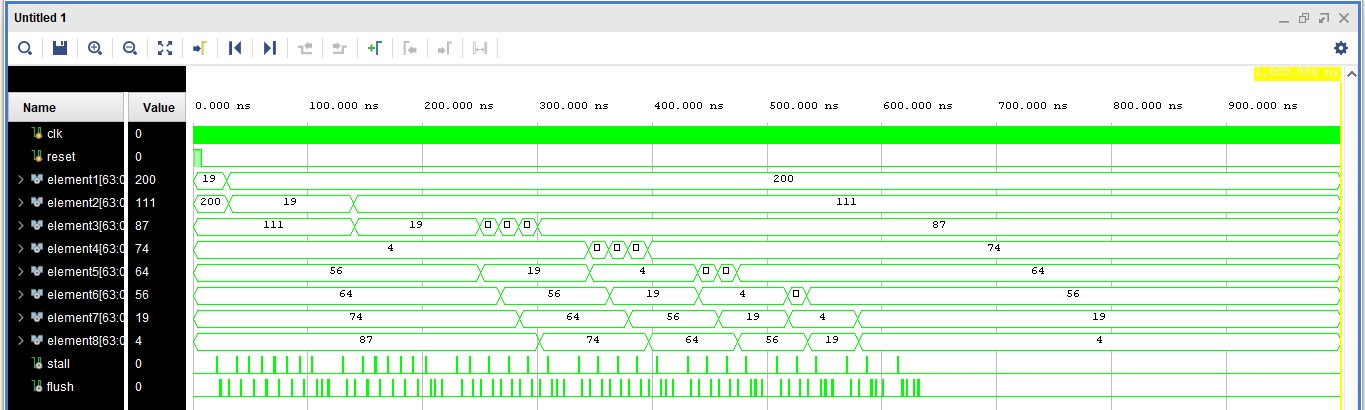
\includegraphics[width=1\textwidth]{task 3 simulation.jpg} 
    \caption{Simulation Output} 
    \label{fig:Output 4} 
\end{figure}
\begin{figure} 
    \centering 
    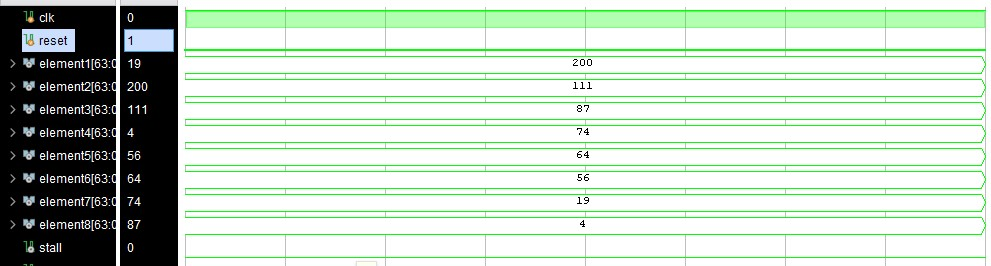
\includegraphics[width=1\textwidth]{task 3 sorted array.jpg} 
    \caption{Sorted Array} 
    \label{fig:Array 2s} 
\end{figure}
\subsection{Changes in Code}
\subsubsection{Hazard Detection Unit}
\begin{lstlisting}[caption={Design Module for Hazard Detection Unit}, captionpos=b, language=RISC-V]
module hazard_detection_unit
  (
    input Memread,
    input [31:0] inst,
    input [4:0] Rd,
    output reg stall
  );
  
  initial
    begin
      stall = 1'b0;
    end
  
  always @(*)
    begin
      if (Memread == 1'b1 && ((Rd == inst[19:15]) || (Rd == inst[24:20])))
        stall = 1'b1;
      else
        stall = 1'b0;
    end
endmodule
\end{lstlisting}
\subsubsection{Flush}
\begin{lstlisting}[caption={Design Module for Flush}, captionpos=b, language=RISC-V]
module pipeline_flush
  (
    input branch,
    output reg flush
  );
  
  initial
    begin
      flush = 1'b0;
    end
  
  always @(*)
    begin
      if (branch == 1'b1)
        flush = 1'b1;
      else
        flush = 1'b0;
    end
  
endmodule
\end{lstlisting}
\subsubsection{Data Extractor}
\begin{lstlisting}[caption={Design Module for Data Extractor}, captionpos=b, language=RISC-V]
module data_extractor
 (
    input [31:0] instruction,
    output reg [63:0] imm_data
  );
  
  always @(*)
    begin
      case (instruction[6:5])
       2'b00:
          begin
            imm_data[11:0] = instruction[31:20];
          end
        2'b01:
          begin
            imm_data[11:0] = {instruction[31:25], instruction[11:7]};
          end
        2'b11:
          begin
            imm_data[11:0] = {instruction[31], instruction[7], instruction[30:25], instruction[11:8]};
          end
      endcase
      imm_data = {{52{imm_data[11]}},{imm_data[11:0]}};
    end  
  
endmodule
\end{lstlisting}
\section{Comparison between Pipelined and non-Pipelined
Single Cycle Processor}
The pipelined RISC-V processor requires 800 nanoseconds to finish executing the bubble sort algorithm, in contrast to the single-cycle processor, which completes the same task in 990 nanoseconds. 

A non-pipelined processor executes each instruction in a sequential manner, meaning it completes one instruction completely before moving on to the next. This can lead to inefficiencies because there may be unused portions of the processor during the execution of an instruction. On the other hand, a pipelined processor breaks down the execution of each instruction into several stages and allows multiple instructions to be processed at the same time. As a result, there is no idle time for the processor, and instructions are executed more quickly.

In practical terms, if we have a pipelined processor and assume that each stage takes the same amount of time, we can calculate the clock cycle of our pipelined processor by dividing the unpipelined cycle time per instruction by the number of stages. For example, if the unpipelined cycle time is 5ns and there are 5 stages, the pipelined processor should have a clock cycle of 1ns. However, if we keep the clock cycle time at 5ns in the pipelined version, it means that each individual module takes 5ns to execute, so the unpipelined version would take 5 times longer, or 25ns, for each instruction.


\section{Challenges // Conclusion}
Building the processor was challenging. The primary goal of pipelining was to enhance the processor's efficiency, enabling the execution of multiple tasks simultaneously. We encountered numerous issues with simulations and the integration of stalls at critical points, making it difficult to sustain the simulation throughout. Additionally, incorporating branch conditions proved challenging due to complexity and dependency issues, yet we managed to develop a pipelined processor that addressed the hazards. The project required extensive debugging of code and modules to identify and fix problems. Ultimately, our processor successfully sorted an unsorted array using the Bubble Sort algorithm. Despite various challenges, we overcame them and created a more efficient multi-cycle, pipelined processor compared to its single-cycle counterpart.


\section{Task Division}
The single-cycle processor was implemented by all the team members combined, while Ahtisham and Hammad incorporated the pipeline stages, hazard detection, and forward-ing unit to the non-pipelined processor. Each member performed their part of the project on time efficiently.
\section{Github Repository}
\href{https://github.com/bilalahmedss/CA-Project}{https://github.com/bilalahmedss/CA-Project}

\end{document}
 
